87. \begin{figure}[ht!]
\center{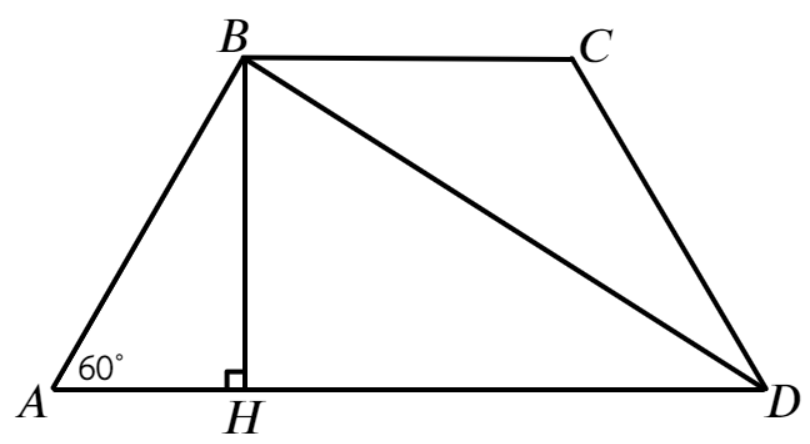
\includegraphics[scale=0.35]{g9-87.png}}
\end{figure}\\
Пусть $AB=BC=CD=x,$ тогда $2x\cos(60^\circ)+x=12,\ 2x=12,\ x=6.$ Найдём $AH=(12-6):2=3,\ BH=3tg(60^\circ)=3\sqrt{3},\ HD=12-3=9,\ BD=\sqrt{27+81}=6\sqrt{3}.$ Описанная вокруг трапеции $ABCD$ окружность является также и описанной окружностью треугольника $ABD,$ значит по теореме синусов $\cfrac{BD}{\sin(60^\circ)}=2R,\ \cfrac{6\sqrt{3}}{\cfrac{\sqrt{3}}{2}}=2R,\ R=6.$\\
